% -----------------------------------------------
% Template for ISMIR Papers
% 2026 version, based on previous ISMIR templates

% Requirements :
% * 6+n page length maximum
% * 10MB maximum file size
% * Copyright note must appear in the bottom left corner of first page
% * Clearer statement about citing own work in anonymized submission
% (see conference website for additional details)
% -----------------------------------------------

\documentclass{article}
\usepackage[T1]{fontenc}
\usepackage[utf8]{inputenc}
\usepackage[submission]{ismir} % Remove the "submission" option for camera-ready version
\usepackage{amsmath,cite,url}
\usepackage{graphicx}
\usepackage{color}
\usepackage{subcaption}
\usepackage{arydshln}
\usepackage{multirow}
\usepackage{booktabs}
\usepackage{blindtext}

\usepackage{tabularx,ragged2e,array} % add to preamble
\newcolumntype{Y}{>{\arraybackslash}X}
\newcolumntype{Z}[1]{>{\arraybackslash}p{#1}}

% Title. Please use IEEE-compliant title case when specifying the title here,
% as it has implications for the copyright notice
% ------
\title{"More than words": Genre-Discriminating Lyrical Patterns in Anglophone German Popular Music}

% Note: Please do NOT use \thanks or a \footnote in any of the author markup

% Single address
% To use with only one author or several with the same address
% ---------------
\oneauthor
  {Anonymous Authors}
  {Anonymous Affiliations\\\texttt{anonymous@ismir.net}}

% Two addresses
% --------------
%\twoauthors
%   {First author} {School \\ Department}
%   {Second author} {Company \\ Address}

% Three addresses
% --------------
% \threeauthors
%   {First Author} {Affiliation 1 \\ \texttt{author1@ismir.edu}}
%   {Second Author} {Affiliation 2 \\ \texttt{author2@ismir.edu}}
%   {Third Author} {Affiliation 3 \\ \texttt{author3@ismir.edu}}

% Four or more addresses
% OR alternative format for large number of co-authors
% ------------
% \multauthor
%   {First author$^1$ \hspace{1cm} Second author$^1$ \hspace{1cm} Third author$^2$}
%   {{\bf Fourth author$^3$ \hspace{1cm} Fifth author$^2$ \hspace{1cm} Sixth author$^1$}\\
%   $^1$ Department of Computer Science, University, Country\\
%   $^2$ International Laboratories, City, Country\\
%   $^3$ Company, Address\\
%   {\tt\small CorrespondenceAuthor@ismir.edu, PossibleOtherAuthor@ismir.edu}
%   }

% For the author list in the Creative Common license, please enter author names.
% Please abbreviate the first names of authors and add 'and' between the second to last and last authors.
\def\authorname{Ananymous Authors}
% \def\authorname{M. Radke and S. Lepa}

% Optional: To use hyperref, uncomment the following.
% \usepackage[bookmarks=false,pdfauthor={\authorname},pdfsubject={\pdfsubject},hidelinks]{hyperref}
% Mind the bookmarks=false option; bookmarks are incompatible with ismir.sty.

\sloppy % please retain sloppy command for improved formatting

\begin{document}

\maketitle

\begin{abstract}
  %max 200 words
Recent advances in natural language processing have improved lyrics-based music genre classification through large language models, yet such black box systems obscure the linguistic structures that actually differentiate music genres. Earlier research in popular music studies, meanwhile, has often emphasized thematic readings of lyrics from single songs without systematically tracing recurrent patterns of idiomatic expressions—leaving stylistic genre differences under-researched until now. Our study bridges these perspectives by uncovering genre discriminative lyrical patterns—topics, sentiments, and idiomatic expressions—in fifty years of Anglophone German popular music. Using the POPTRAG corpus and \textit{Discogs} genre annotations for 126,042 tracks with English lyrics, we apply the fightin' words method to  identify statistically distinctive n-grams across genres and build interpretable topic, sentiment, and expression dictionaries. Finally, we cluster the n-grams contained in each dictionary via structural topic modeling using target genres as prevalence priors. Resulting interpretable lyrics features are employed in machine-learning models that reveal how topics, sentiments, and idiomatic expressions function as stylistic markers for single popular music genres. Our transparent ML approach retains roughly 80\% of the predictive performance of a transfer-learned DistilBERT classifier while offering conceptual insight into how lyrics encode genre identity. 
\end{abstract}


\section{Introduction}\label{sec:introduction}


% Warum nciht textuelle Statistik; wie werden topic models und sentimente in der KoWi gefasst (nomen, Adjektive); was ist idiomatic expressions

Given these considerations we pose the following research questions:

\noindent
\begin{tabularx}{\linewidth}{@{}Z{0.08\linewidth} Y@{}}
\textbf{RQ1} & Which content-related genre-discriminative lyrical patterns (topics, sentiments, idiomatic expressions) exist in Anglophone German popular music? \\
\textbf{RQ2} & To what extent do pattern-based interpretable ML models match a fine-tuned transformer baseline on popular music genre prediction? \\
\textbf{RQ3} & What can we learn about lyrical genre differences from such interpretative models for popular music studies? \\
\end{tabularx}



\section{Methods}
\subsection{Corpus and Genre Annotations}
For our analysis, we relied on the POPTRAG corpus of 254,334 unique popular tracks released and frequently listened to in Germany over the past 50 years. The corpus combines multiple sources: (1) 215,702 tracks from weekly \textit{MediaControl} German single and album charts, capturing the 100 most relevant albums and songs per week by physical/digital sales, streams, and broadcasts (18 Nov 1977–21 Nov 2024; limited to 75\% of tracks successfully linked to Spotify identifiers for consistent metadata); (2) 11,994 unique track entries from Germany's Daily Top 200 Spotify charts (Jan 2017–Nov 2024). To capture not only sold music but also listened-to music no longer in the charts, the corpus additionally includes (3) 26,949 Spotify track recommendations from 126 German-market genre seeds (retrieved 29 Nov 2024; median 325 per seed, IQR 25, range 49–343); and (4) 8,801 tracks from the 100 top-featured Spotify playlists for Germany (retrieved 29 Nov 2024, median 90 tracks per playlist, IQR 42, range 28–750). 853 tracks shorter than 30 seconds were excluded and only unique title-artist combinations were retained, selecting earlier release dates for duplicates.

\begin{figure}
  \centering
  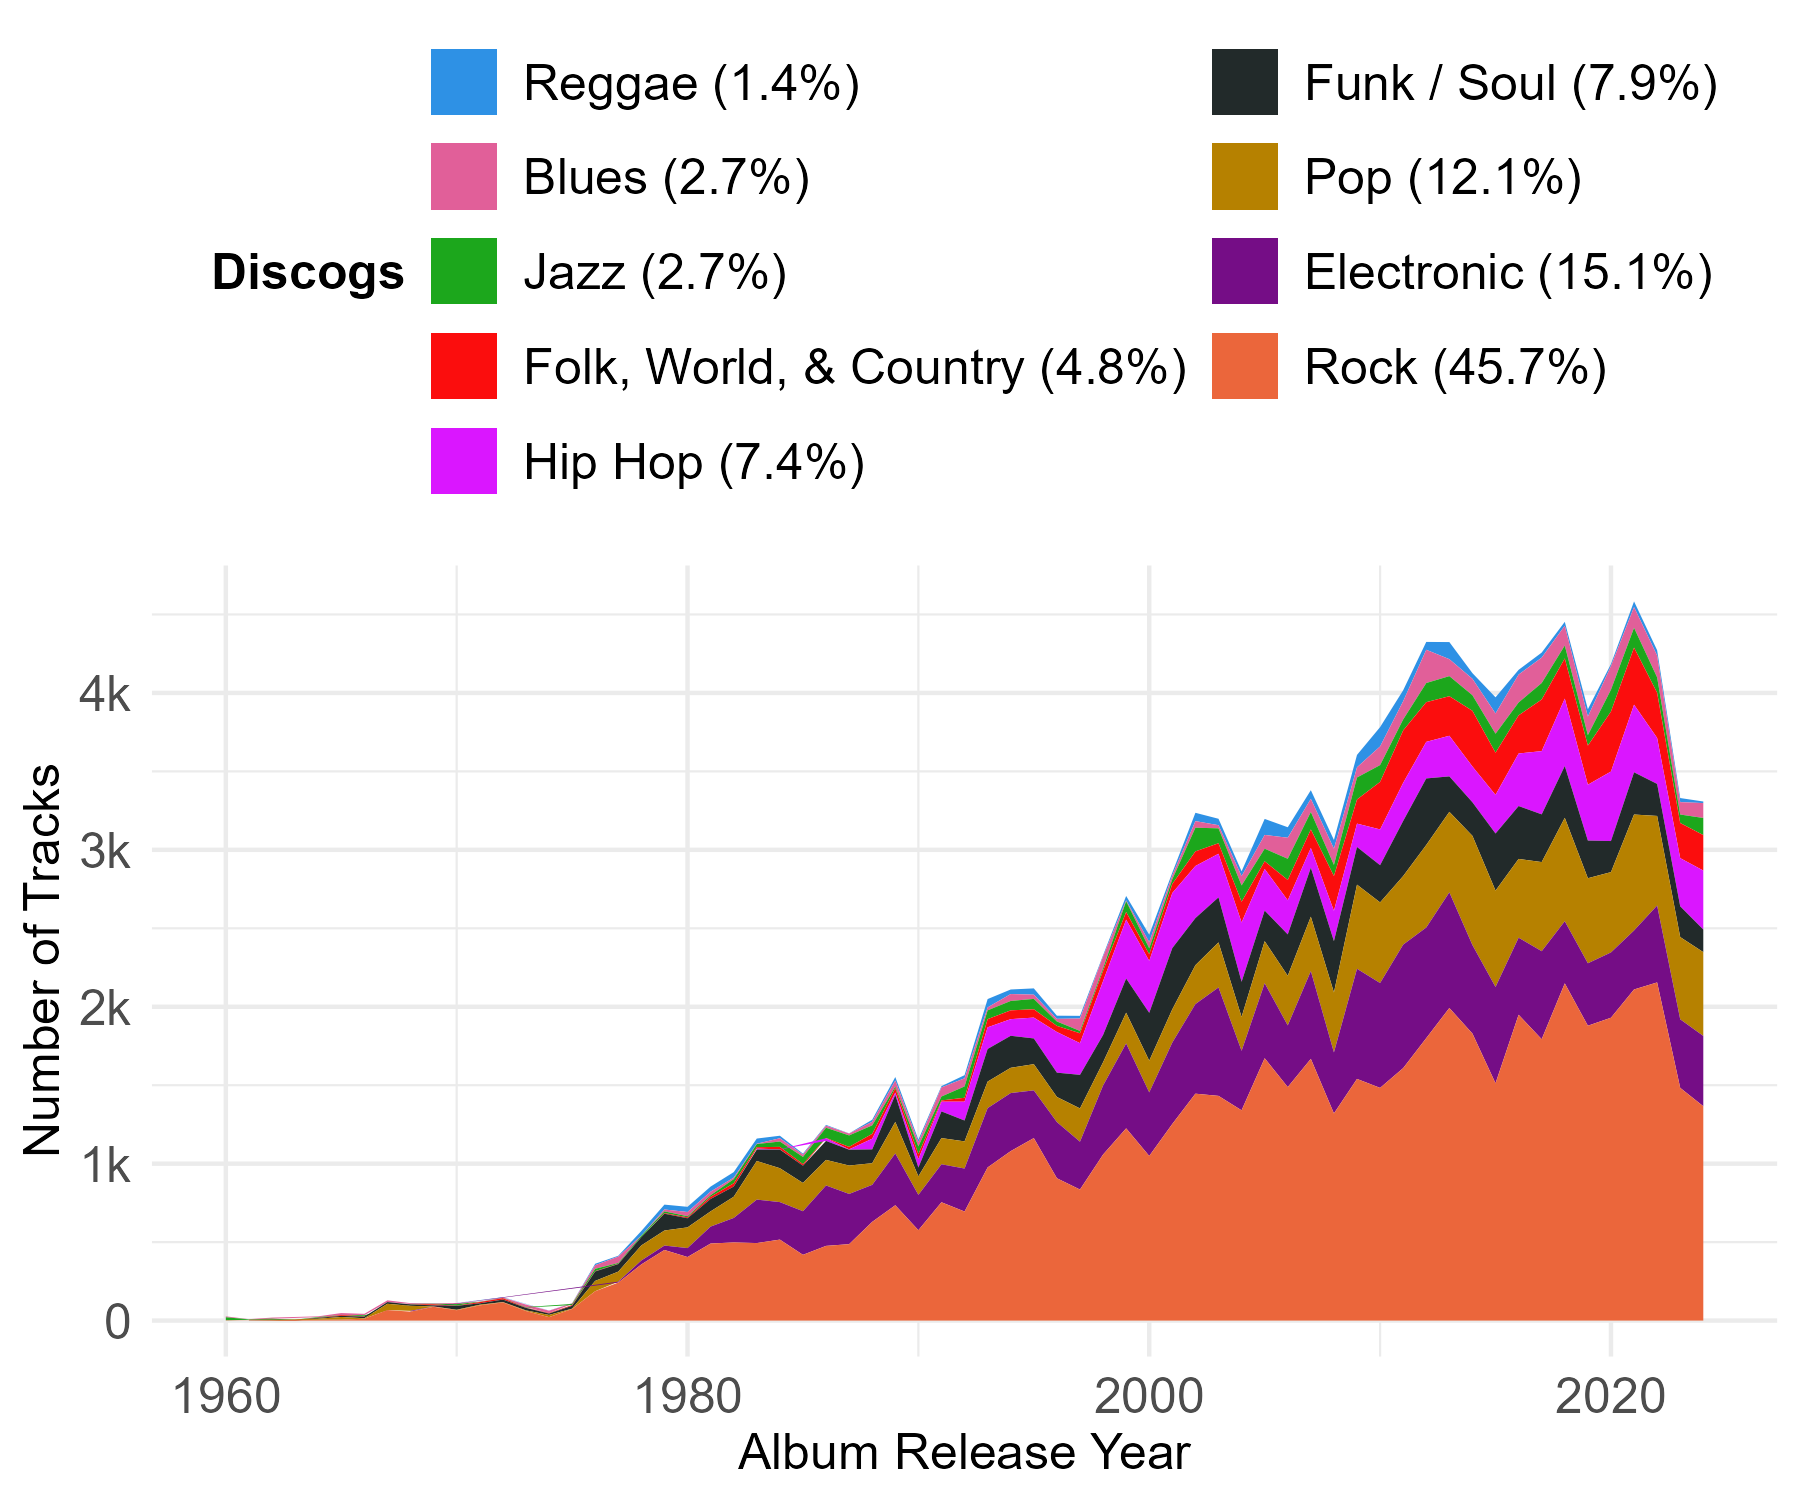
\includegraphics[alt={Corpus description},width=\linewidth]{figures/corpus_descriptive.png}
  \caption{Composition of the analyzed corpus.}
  \label{fig:corpus}
\end{figure}


Employing data linkage and webscraping, we enriched POPTRAG with lyrics from \textit{Genius} and release genre annotations from \textit{Discogs} for the tracks in the corpus. For our analysis, we focused on tracks with retrieved English lyrics and at least one \textit{Discogs} genre annotation (51\%). For 35\% of these remaining tracks, that were assinged more than one genre by the \textit{Discogs} community, we retained only the most specific genre label (i.e., the one that appeared least frequently in the corpus) to enable an easily interpretable single-label classification task. Finally, we removed genres that made up less than 1\% of the remaining corpus, resulting in a final sample of N=126,042 tracks across 9 genres (see Figure \ref{fig:corpus} for details on the corpus composition).


\subsection{Genre Disrciminating Vocabularies}
% Figure \ref{fig:method_flow} gives an overview of the complete method flow. 
Please refer to Figure X
 % TODO
for an overview of the method flow; all operations that involved randomness were seeded with 42 for reproducibility. In order to identify genre-discriminating lyrical patterns (RQ1), we first performed basic cleaning on the raw lyrics data form \textit{Genius} by: trimming whitespaces, removing everything between and including square brackets, normalizing asterisks, removing repetition and song position indicators, and fixing missing apostrophes (e.g., ``don t'' $\rightarrow$ ``don't''). 

Our aim was to exctract relevant n-grams for each type of lyrical pattern: topics, sentiments, and idomatic expressions. Depending on the type of pattern, we applied different preprocessing steps, reducing the lyrics to relevant tokens. For topics and semantics ngrams, we exapanded contractions in the lyrics (e.g., ``don t'' $\rightarrow$ ``do not''), lemmatized and POS-tagged the lyrics using \textit{spaCy's} \texttt{en\_core\_web\_lg} model in combination with an additional custom domain lexicon for lemmatization, and reduced the lyrics to nouns for topics and adjectives and adverbs for sentiments. For topics and sentiments, we only kept tokens with more than two characters that were contained in both the vocabulary that \texttt{en\_core\_web\_lg} was trained on and the English vocabulary of the \textit{nltk} library to exclude non-lexical items. After preprocessing, we split the corpus into a training set (80\%) and a holdout set (20\%) stratified by genre for all subsequent analyses. Me made sure that there was no artist overlap when splitting to mitigate artist and album effects \cite{flexerEffectsAlbumArtist2010}. 

The following steps were then applied to the training corpus only, and the holdout set was only used for evaluation of the final ML models. In the next step, we build the three seperate vocabularies of genre-discriminating n-grams for topics, sentiments, and idiomatic expressions. For topics and sentiments, we extracted all unigrams, and for idiomatic expressions, we extracted all n-grams (n=1-4). All n-grams had to appear with more than one artist in the corpus to be included in the respective vocabulary. We removed all n-grams from the candidates that contained stopwords only and for expressions also removed bigrams that start with ``a'', ``an'', ``the'', and ``to'', to exclude trivial bigrams: infinitives and nouns with articles.

Then, for the remaining sets of ngrams (topics, sentiments, and expressions), we applied the fightin' words method \cite{monroeFightinWordsLexical2017} to identify genre discriminative n-grams within the set. This method quantifies how strongly each n-gram is associated with a particular genre by computing log-odds ratios—a measure comparing the relative frequency of an n-gram in one genre versus all others combined. To account for rare n-grams that may appear by chance in small samples, we applied Bayesian smoothing using empirical prevalence as a Dirichlet prior, which adds a penalty to extremely infrequent observations. We then converted these log-odds ratios into z-scores, standardized test statistics that indicate how many standard deviations an n-gram's association strength deviates from zero; larger absolute z-scores indicate stronger genre discrimination. To convert z-scores to p-values, we applied a one-sided statistical test (upper tail), which identifies n-grams significantly associated with each genre. Since we computed z-scores for thousands of n-grams simultaneously across all genres, we applied Benjamini-Hochberg false discovery rate (FDR) correction \cite{benjaminiControllingFalseDiscovery1995} at $\alpha = 0.001$. This procedure identifies the most stringent z-score threshold where at most 0.1\% of significant findings are expected to be false positives, controlling for multiple testing. N-grams passing this FDR-corrected threshold (corresponding to $p < 0.001$) with positive z-scores were retained in the final vocabularies. 


\subsection{Genre Discriminating Topics, Sentiments, and Idiomatic Expression Types}
To identify genre-discriminating latent topics, sentiments, and types of idiomatic epxressions (RQ1), we employed structural topic modeling (STM) \cite{robertsStmPackageStructural2019} on the train corpus using the n-grams contained in the respective vocabularies. We used the target genres as prevalence priors to guide the clustering of n-grams into latent types that are discriminative for specific genres. To mitigate sparsitiy during model training, we aggregated the n-gram counts at the artist level, again selecting the most specific genre for artists with multiple genres for the prevalence priors. 

We ran STM separately for topics, sentiments, and expressions, testing a range of 2 to 20 types for, that allowed for interpretable solutions. For determining the number of topics, we used a train-validation split and calculated semantic coherence and likelihood on the validation set as well as the exclusivity score \cite{robertsStructuralTopicModels2014} for each number of types. We determined the optimal number of types primarily based on the highest exclusivity score, which measures how uniquely n-grams are associated with a single type, while also striving for good validation semantic coherence (i.e., how well the top n-grams in a type cohere semantically) and high likelihood on validation data. After selecting the optimal number of types, we reran the STM on the full training corpus and interpreted and labeled the clusters based on the n-grams with the highest FREX scores \cite{bischofSummarizingTopicalContent2012}, which balance frequency and exclusivity to identify representative n-grams for each type. Finally, we calculated the probabilities of each topic, sentiment, and expression type per genre (i.e., the mean of topic proportions accros the genre) in the training data to analyze their distribution across genres.

\subsection{Machine Learning Experiments}
To evaluate the predictive performance of the identified genre-discriminating lyrical patterns (RQ2), we trained machine learning models to predict music genre based on the extracted topics, sentiments, and expression types as features. We compared the performance of these interpretable models to a random baseline, a traditional TF-IDF \cite{fell2014lyrics} + GLMNET \cite{defazioSAGAFastIncremental2014} pipeline, and a fine-tuned DistilBERT model \cite{sanhDistilBERTDistilledVersion2020} trained directly on raw lyrics. For a direct comparison to the TF-IDF + GLMNET pipeline, we first trained GLMNET \cite{defazioSAGAFastIncremental2014} models with fixed hyperparameters (penalty C=1, L1 regularization ratio=0.5) on each individual feature set (topics, sentiments, expressions) as well as on a combined feature set that included all three types of features. Then, we performed systematic hyperparameter tuning for the combined features GLMNET model (10x10 grid search, C logarithmic in [1e-5, 1e-5], L in [0, 1]) and a LightGBM \cite{keLightGBMHighlyEfficient2017a} model (Tree-structured Parzen Estimator \cite{optuna2019}, number of tress in [100, 2000], learning rate in [0.001, 0.1], number of leaves in [20, 70], max depth of trees in [1, 10], minimum data in leaf in [1, 100], feature fraction at split in [0.1, 1.0], L1 and L2 regularization logarithmic in [1e-8, 10.0] respecitively) with 4-fold artist grouped and stratified cross validation to ensure optimal parameterization and to assess whether more flexible models could further improve performance while retaining interpretability. We evaluated model performance using macro F1 scores from 4-fold cross-validation on the training set and on the holdout set, which was not used for any part of the model training or feature extraction process.

To show wich features contribute most to genre prediction and to inspect individual genre profiles (RQ3), we computed the permutation feature importance \cite{fisherAllModelsAre2019} on the holdout set for the best performing combined features model. Moreover, we computed SHAP values \cite{lundbergUnifiedApproachInterpreting2017a} with the holdout set for  the genre with the best performance to show how specific features contribute to genre prediction for this genre in particular.


\section{Results}

% RQ1: Welche inhaltlichen genre-discriminativen lyrischen Muster (Themen, Sentiments, idiomatische Ausdrücke) existieren in der anglophonen deutschen populären Musik?
\subsection{Genre Disrciminating Patterns}
Using the fightin' words method, we identified topic, sentiment, and idiomatic expressions vocabulary lists containing n-grams that are statistically significant for distinguishing between popular music genres in our training corpus. The topic vocabulary comprises 3,831 nouns, the sentiment vocabulary includes 857 adjectives and adverbs. The expressions vocabulary contains 56,804 idiomatic expressions (12\% unigrams, 33\% bigrams, 35\% trigrams, and 19\% quadgrams).

\begin{table*}[!t]
  \setlength{\tabcolsep}{6pt}
  \centering
  \footnotesize
  \begin{tabular}{l l l}
    \toprule
    Type  & Label & Example high-FREX n-grams \\
    \midrule
    Topic & Americana & beer, john, funk, monkey, whiskey, jack, cowboy, johnny, hat, lee \\
    Topic & Darkness & chaos, death, humanity, destruction, agony, decay, hate, existence, hatred, terror \\
    \midrule
    Sentiment & ambivalent & pretty, maybe, good, nice, bad, sad, easy, glad, totally, busy \\
    Sentiment & apocalyptic & final, evil, eternal, ancient, sacred, deadly, violent, rotten, mortal \\
    \midrule
    Expression & Christmas Phrases & let it snow let, snow let it snow, it snow let it, lonley so lonly so, dreaming of a white, of a white christmas, \\
    & & a merry little christmas, have yourself a merry, yourself a merry little, in a winter wonderland \\
    Expression & Dance Floor Commands & na na na na, doo doo doo doo, ba ba ba ba, ya ya ya ya, man man man man, li li, ma ma ma ma,\\ 
    & & move your body, put your hands up, ba dum\\
    \bottomrule
  \end{tabular}
  \caption{Example interpretations of genre-discriminative topic, sentiments, and expression types with top high-FREX n-grams.}
  \label{tab:frex_examples}
\end{table*}

Based on these vocabularies, we extracted dense topic, sentiment, and idiomatic expressions features by integrating the n-grams contained in each vocabulary via structural topic modeling into latent types using target genres as prevalence priors, thus getting genre-discriminative topics, sentiments, and types of idiomatic expressions. Within the range from 2 to 20 types, we chose the optimal number of types for each topics, sentiments, and expressions primarily based on the highest exclusivity score, while striving for good semantic coherence and high likelyhood using holdout data (see Appendix for selection curves?). We chose 10 topics, 6 sentiments, and 11 expression types and then interpreted and labeled the clusters based on the n-grams with the highest FREX scores (see Table \ref{tab:frex_examples} for examples, see Appendix for full list). The genre-discriminative topics we identified were: \textit{Americana}, \textit{Darkness}, \textit{Embodiment}, \textit{Existentialism}, \textit{Heroic Saga}, \textit{Holidays}, \textit{Nature}, \textit{Narrative}, \textit{Romance}, and \textit{Street Life}. The genre-discriminative sentiments we identified were: \textit{ambivalent}, \textit{apocalyptic}, \textit{brash}, \textit{nostalgic}, \textit{playful}, and \textit{romantic}. The genre-discriminative expression types we identified were: \textit{Christmas Phrases}, \textit{Dance Floor Commands}, \textit{Denials \& Negotiations}, \textit{Doom Imaginary}, \textit{Jamaican Patois}, \textit{Landscape Imaginary}, \textit{Love Affirmations}, \textit{Nostalgic Formulas}, \textit{Traditional Street Slang}, \textit{Trap Slang}, and \textit{Vocalizations}.


\begin{figure*}[htbp]
  \onecolumn
  \centering
  \begin{subfigure}[b]{0.33\linewidth}
    \centering
    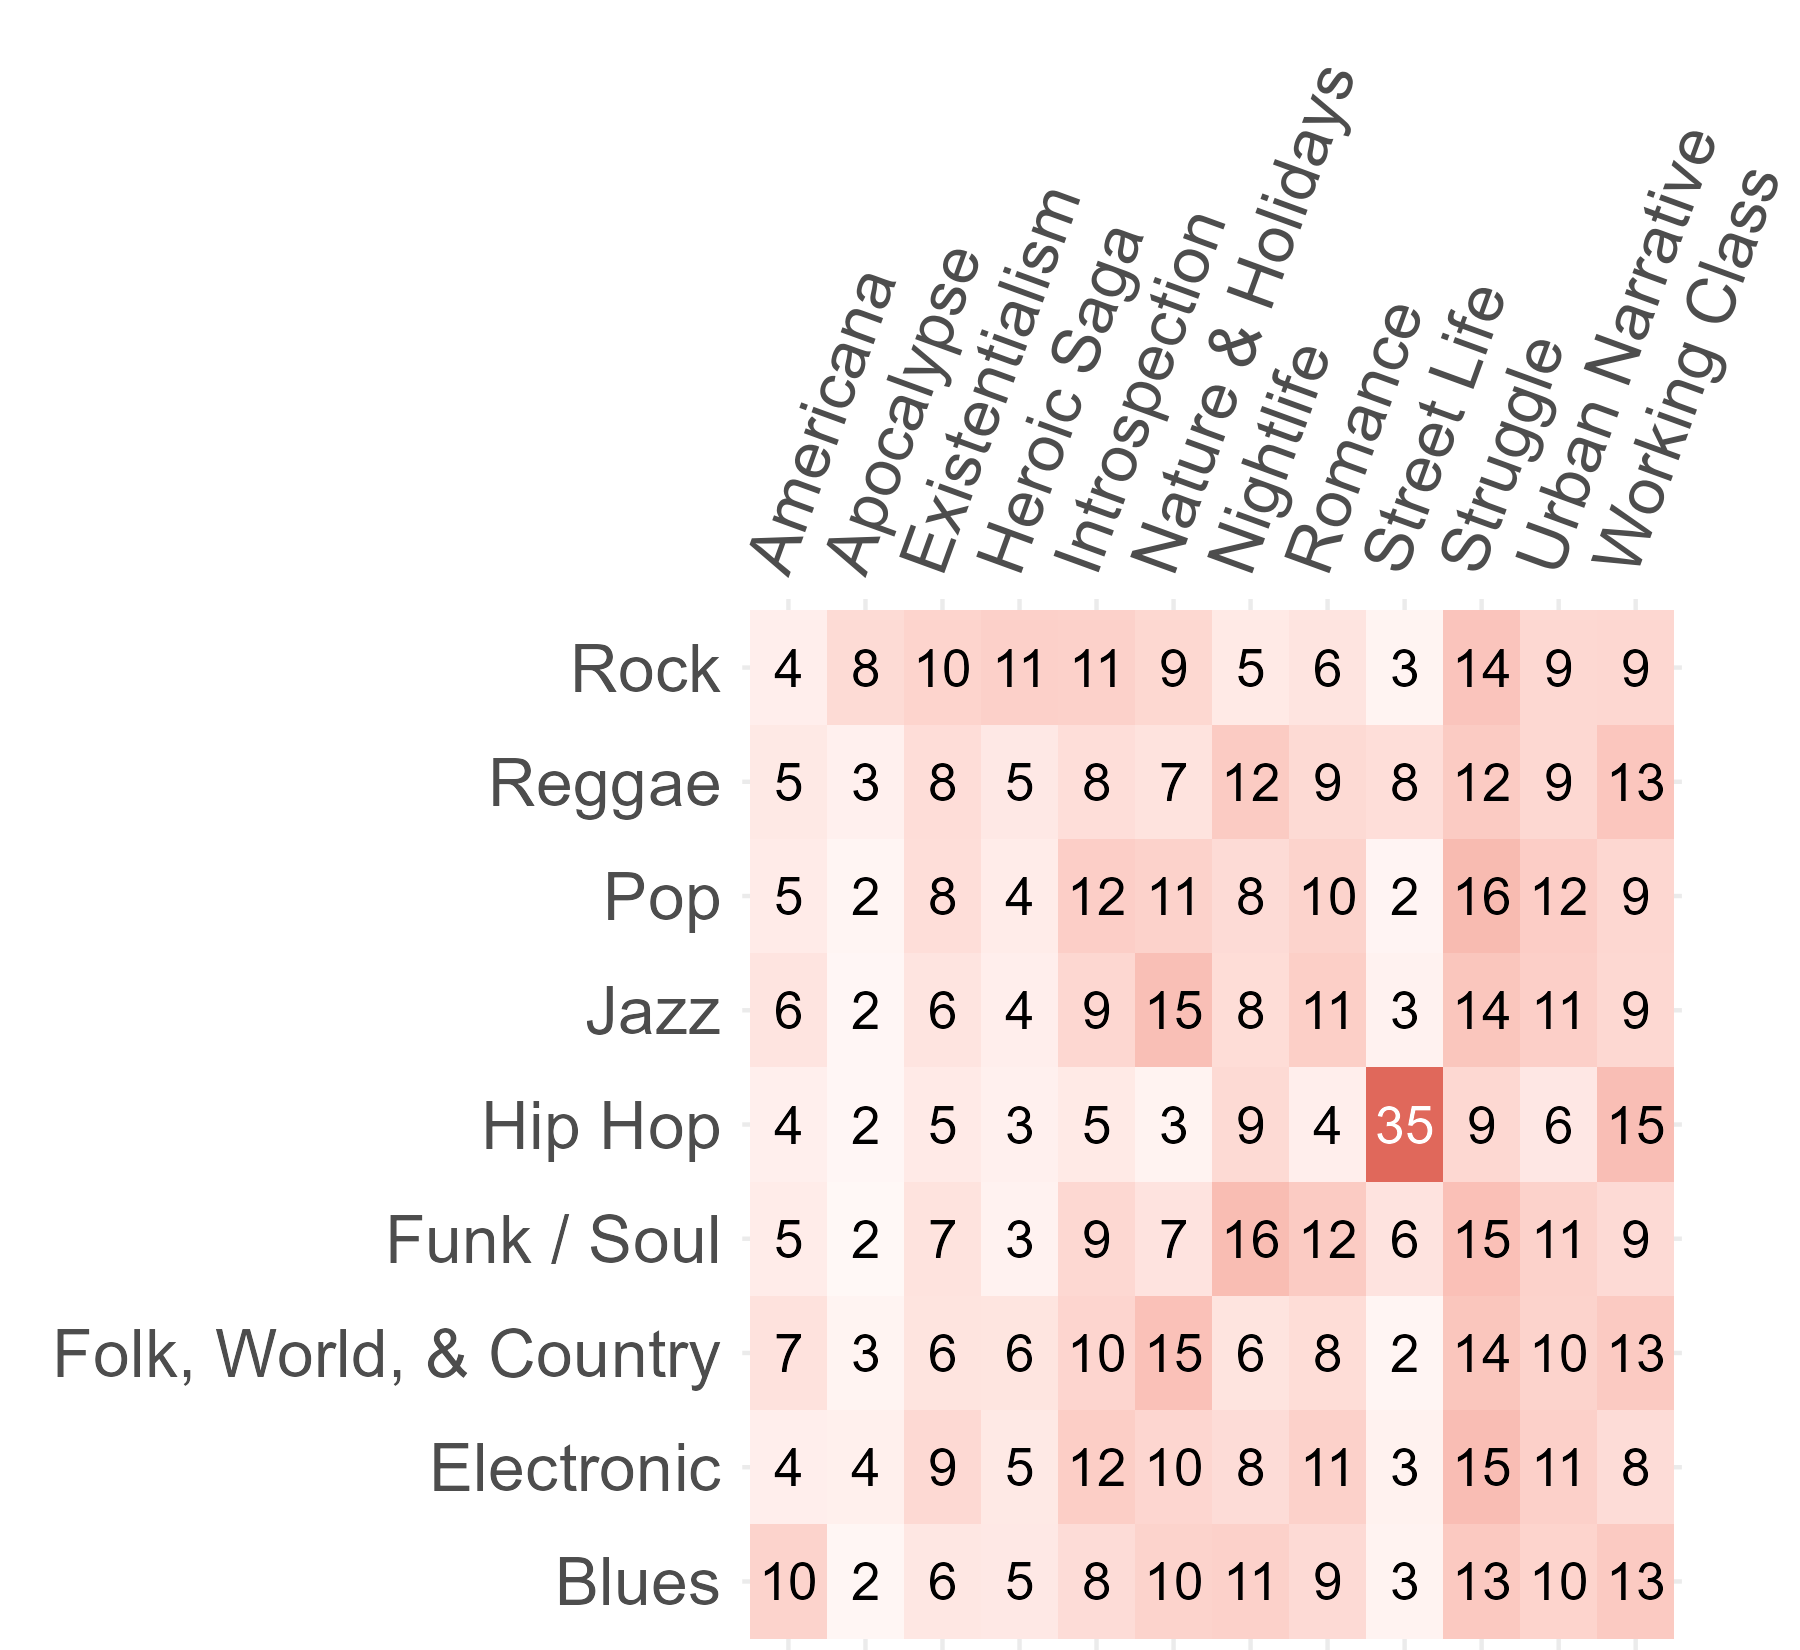
\includegraphics[alt={Topic Heatmap},width=\linewidth]{figures/topic_genre_heatmap_train.png}
    \caption{topics}
    \label{fig:topics}
  \end{subfigure}\hfill
  \begin{subfigure}[b]{0.33\linewidth}
    \centering
    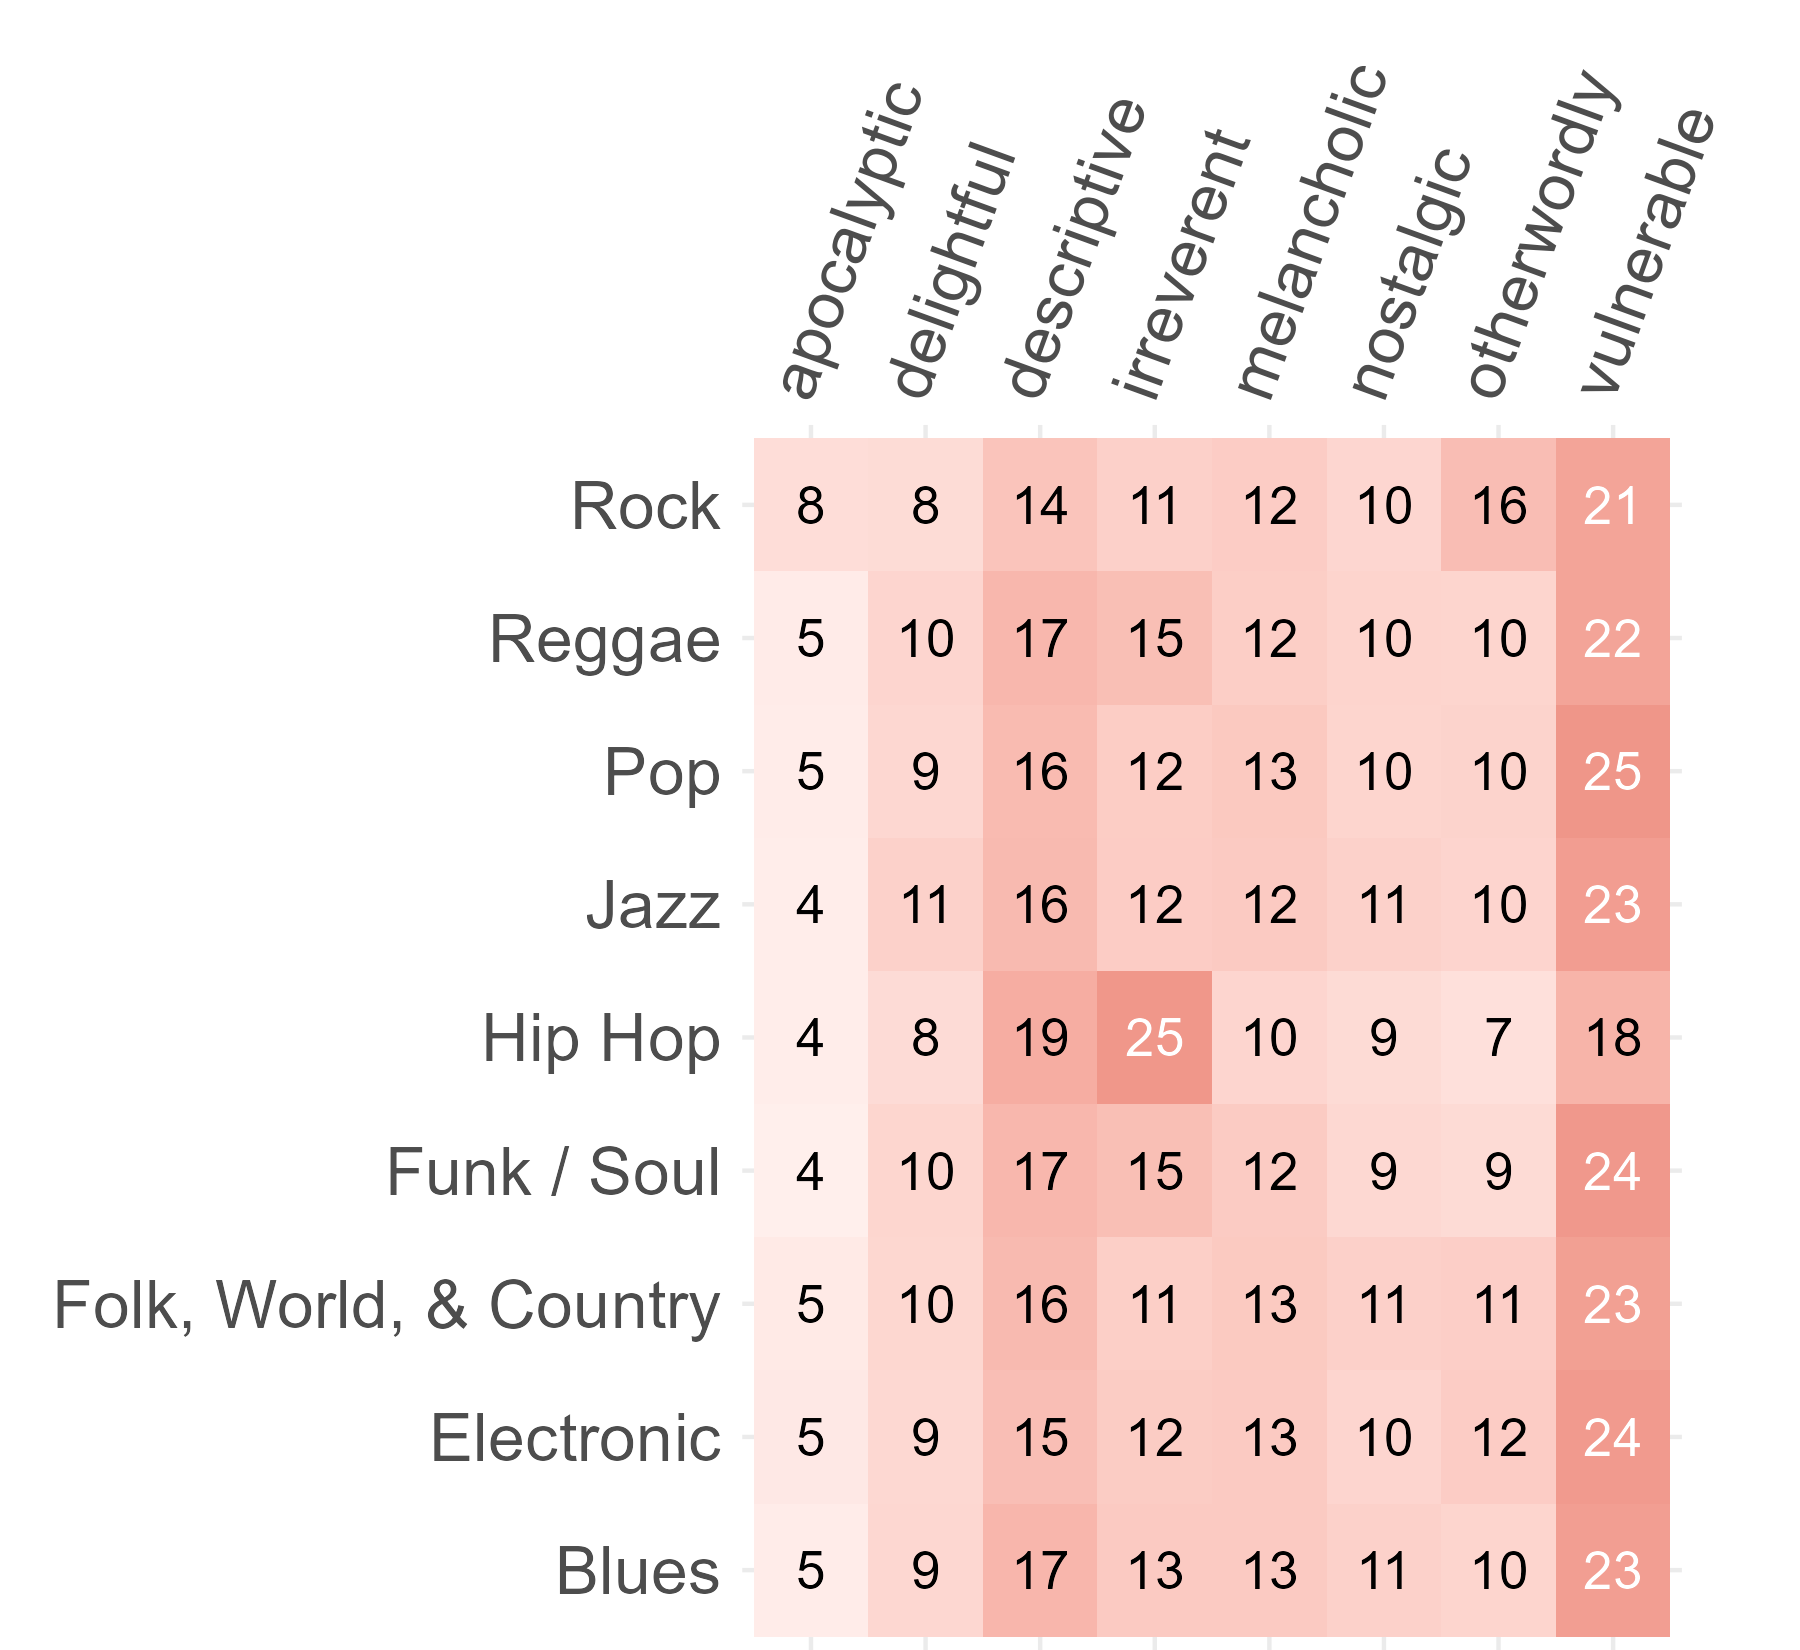
\includegraphics[alt={Style Heatmap},width=\linewidth]{figures/sentiment_genre_heatmap_train.png}
    \caption{sentiments}
    \label{fig:sentiments}
  \end{subfigure}\hfill
  \begin{subfigure}[b]{0.33\linewidth}
    \centering
    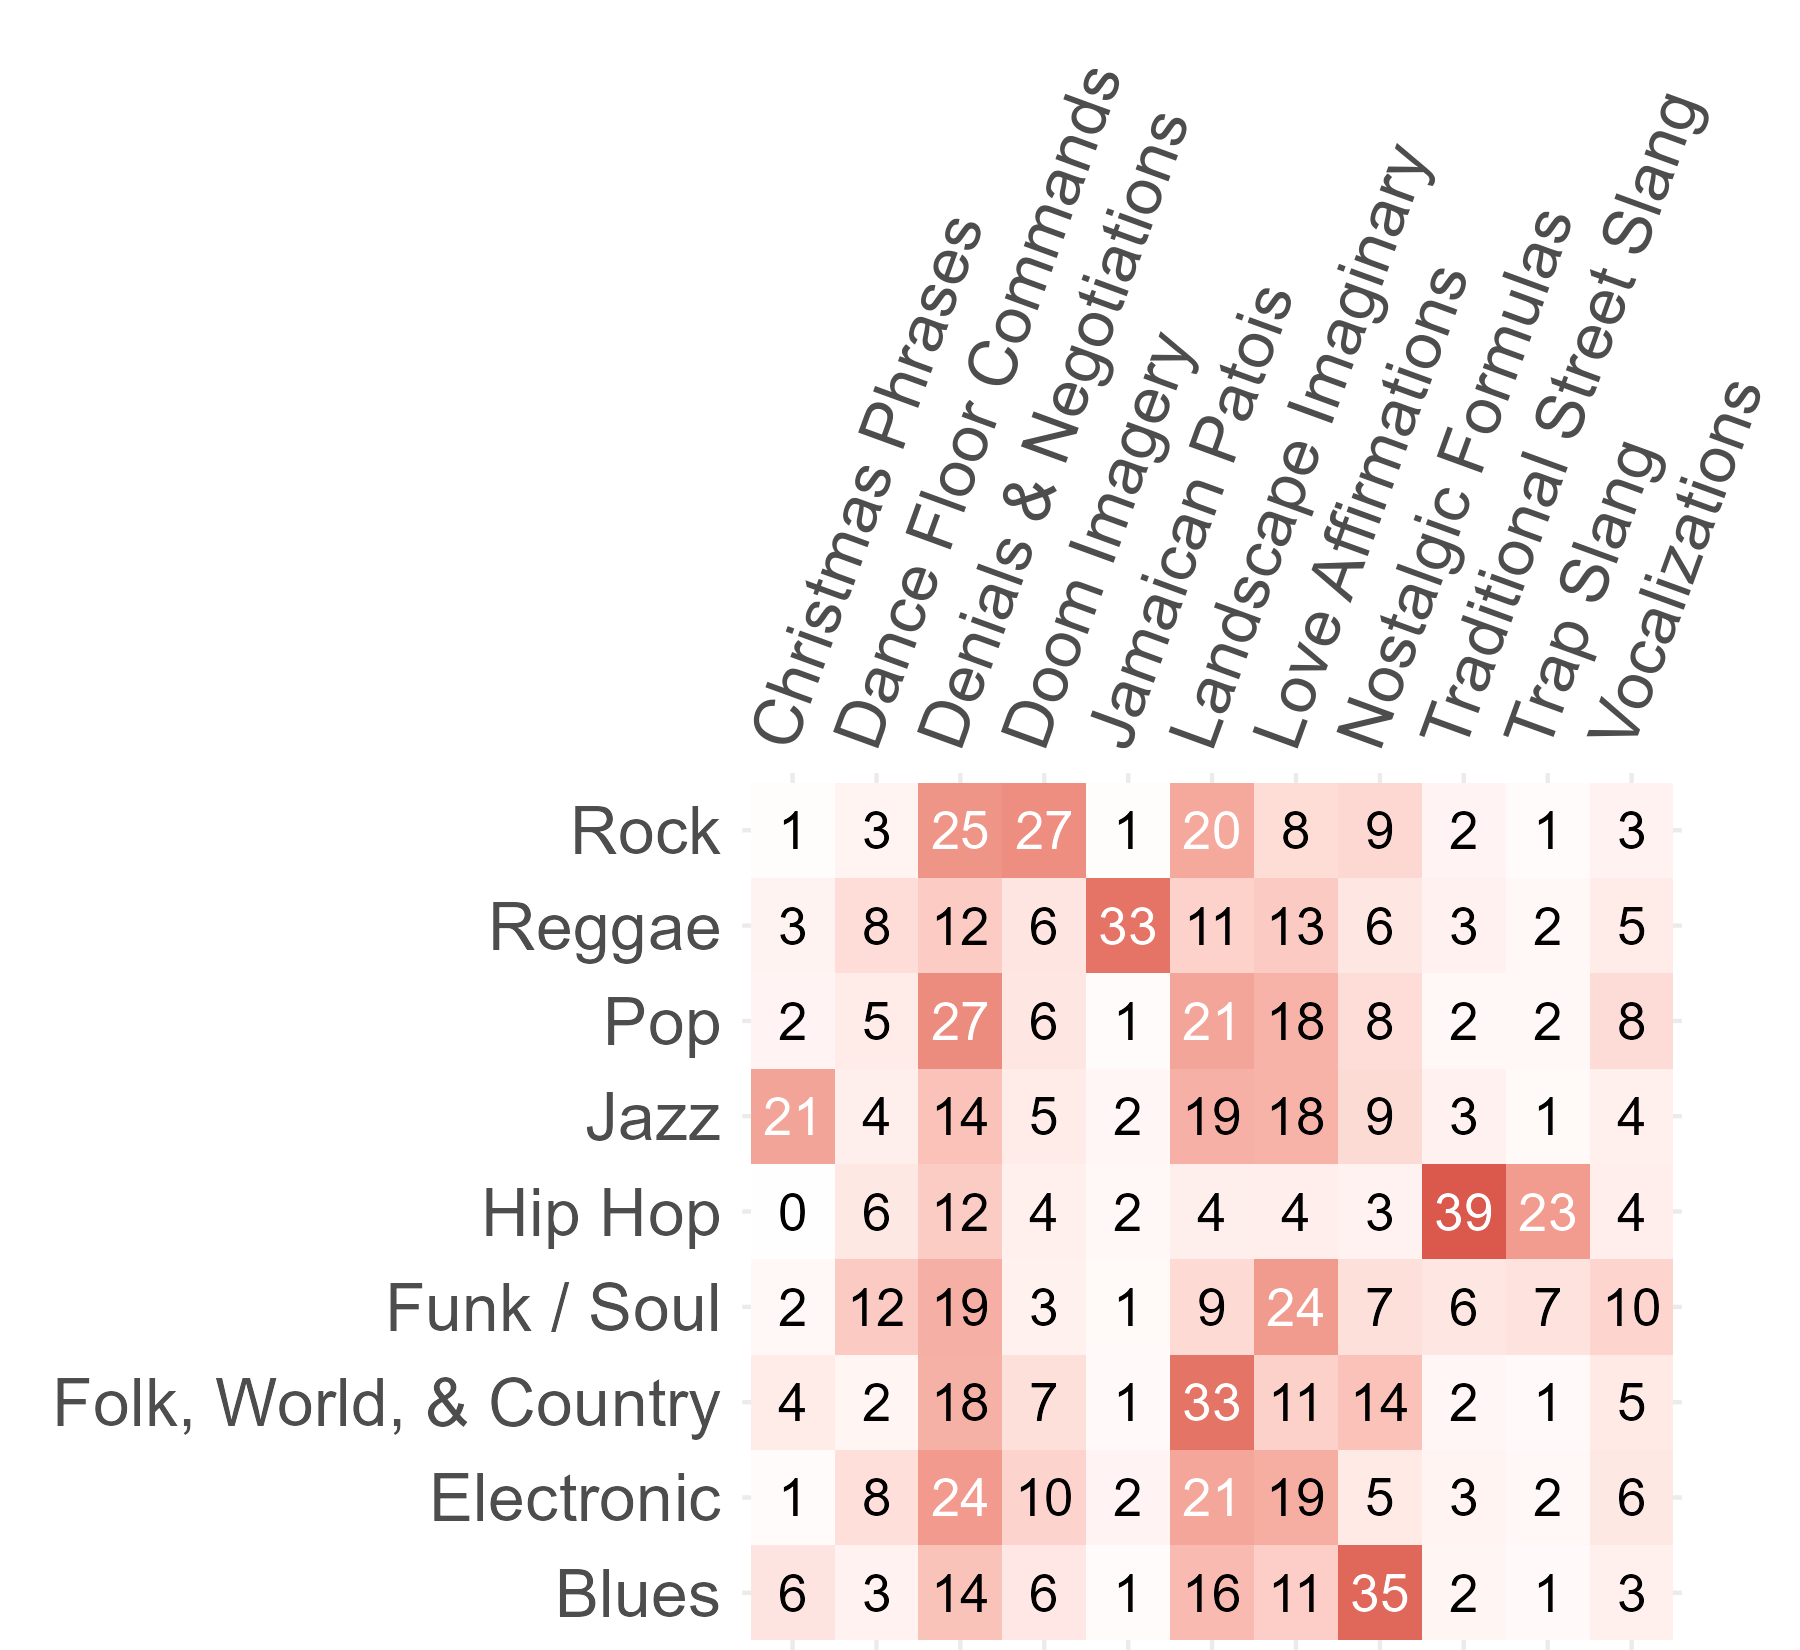
\includegraphics[alt={Style Heatmap},width=\linewidth]{figures/expressions_genre_heatmap_train.png}
    \caption{idiomatic expressions}
    \label{fig:expressions}
  \end{subfigure}
  \caption{Latent genre-discriminative topics, sentiments, and styles: probabilities per genre in the training corpus [\%].}
  \label{fig:heatmaps}
  \twocolumn
\end{figure*}

Finally, we calculated the probabilities of each topic, sentiment, and expression type per genre in the training data to analyze their distribution across genres (see Figure \ref{fig:heatmaps}). Overall, we find similar distributions with small deviations for topics and sentiments. Moreover, while the probabilities for sentiments are distributed more evenly across types, probabilities for topics show more pronounced concentrations in specific genres. \textit{Existentialism} shows comparably high probability for nearly all genres. A notable exception for this general pattern is the \textit{Hip Hop} genre, which shows a particularly high probability for the \textit{Street Life} (41\%) topic and \textit{brash} (28\%) sentiment, while also showing particularly low probabilities for the \textit{Existentialism}(13\%), \textit{Nature} (4\%) and \textit{Romance} (6\%) topic as well as the \textit{romantic} (16\%) sentiment. In addition, \textit{Rock}'s probabilities are particularly high for the \textit{Darkness} (11\%) and \textit{Heroic Saga} (10\%) topics, as well as for the \textit{apocalyptic} (18\%) sentiment. 

The probability distribution of expression types for genres is more heterogeneous than for topics and sentiments, and distributions are more concentrated. Some expression types are particularly concentrated in specific genres, such as \textit{Traditional Street Slang} and \textit{Trap Slang} for \textit{Hip Hop}, \textit{Jamaican Patois} for \textit{Reggae}, \textit{Doom Imaginary} for \textit{Rock}, and \textit{Christmas Phrases} for \textit{Jazz}. However, we also find some expression types that are more evenly distributed across genres, such as \textit{Denials \& Negotiations}, \textit{Landscape Imaginary}, and \textit{Love Affirmations}.

%RQ2: Wie gut performen die pattern-basierten interpretativen ML-Modelle im Vergleich zu einem state of the art tranformer-basierten LLM?
\subsection{Interpretable ML Performance}

\begin{table}
  \footnotesize
  \setlength{\tabcolsep}{5pt}
  \centering
  \begin{tabular}{l l l c c}
    \toprule
    Features & Model & Hyperparameters & $F1_{\text{CV}}$ & $F1_{\text{HO}}$ \\
    \midrule
    Prevalences & Random & — & — & 0.111 \\
    Raw Lyrics & DistillBERT & default & — & 0.374 \\
    TF-IDF & GLMNET & $C$=1, $L1$=0.5 & — & 0.248 \\
    \midrule
    Topics & GLMNET & $C$=1, $L1$=0.5 & — & 0.229 \\
    Sentiments & GLMNET & $C$=1, $L1$=0.5 & — & 0.135 \\
    Expressions & GLMNET & $C$=1, $L1$=0.5 & — & 0.282 \\ 
    Combined & GLMNET & $C$=1, $L1$=0.5 & — & 0.292\\ 
    \midrule
    Combined & GLMNET & $C$=0.002, $L1$=0.33 & 0.335 & 0.291 \\
    Combined & LightGBM & tuned$^\dagger$ & 0.354 & 0.300 \\ 
    \bottomrule
  \end{tabular}
  \caption{Macro $F1$ evaluation for classification experiments. Values show mean $F1$ from 4-fold cross-validation (CV) and $F1$ on holdout set (HO). Dashes indicate models trained with fixed hyperparameters. $^\dagger$LightGBM hyperparameters: 223 estimators, learning rate=0.079, 69 leaves, max depth=9, min 31 data points in leaf, L1 Regularization=$1.43 \times 10^{-2}$, L2 Regularization=$9.15 \times 10^{-5}$.}
  \label{tab:f1}
\end{table}



\begin{figure}
  \centering
  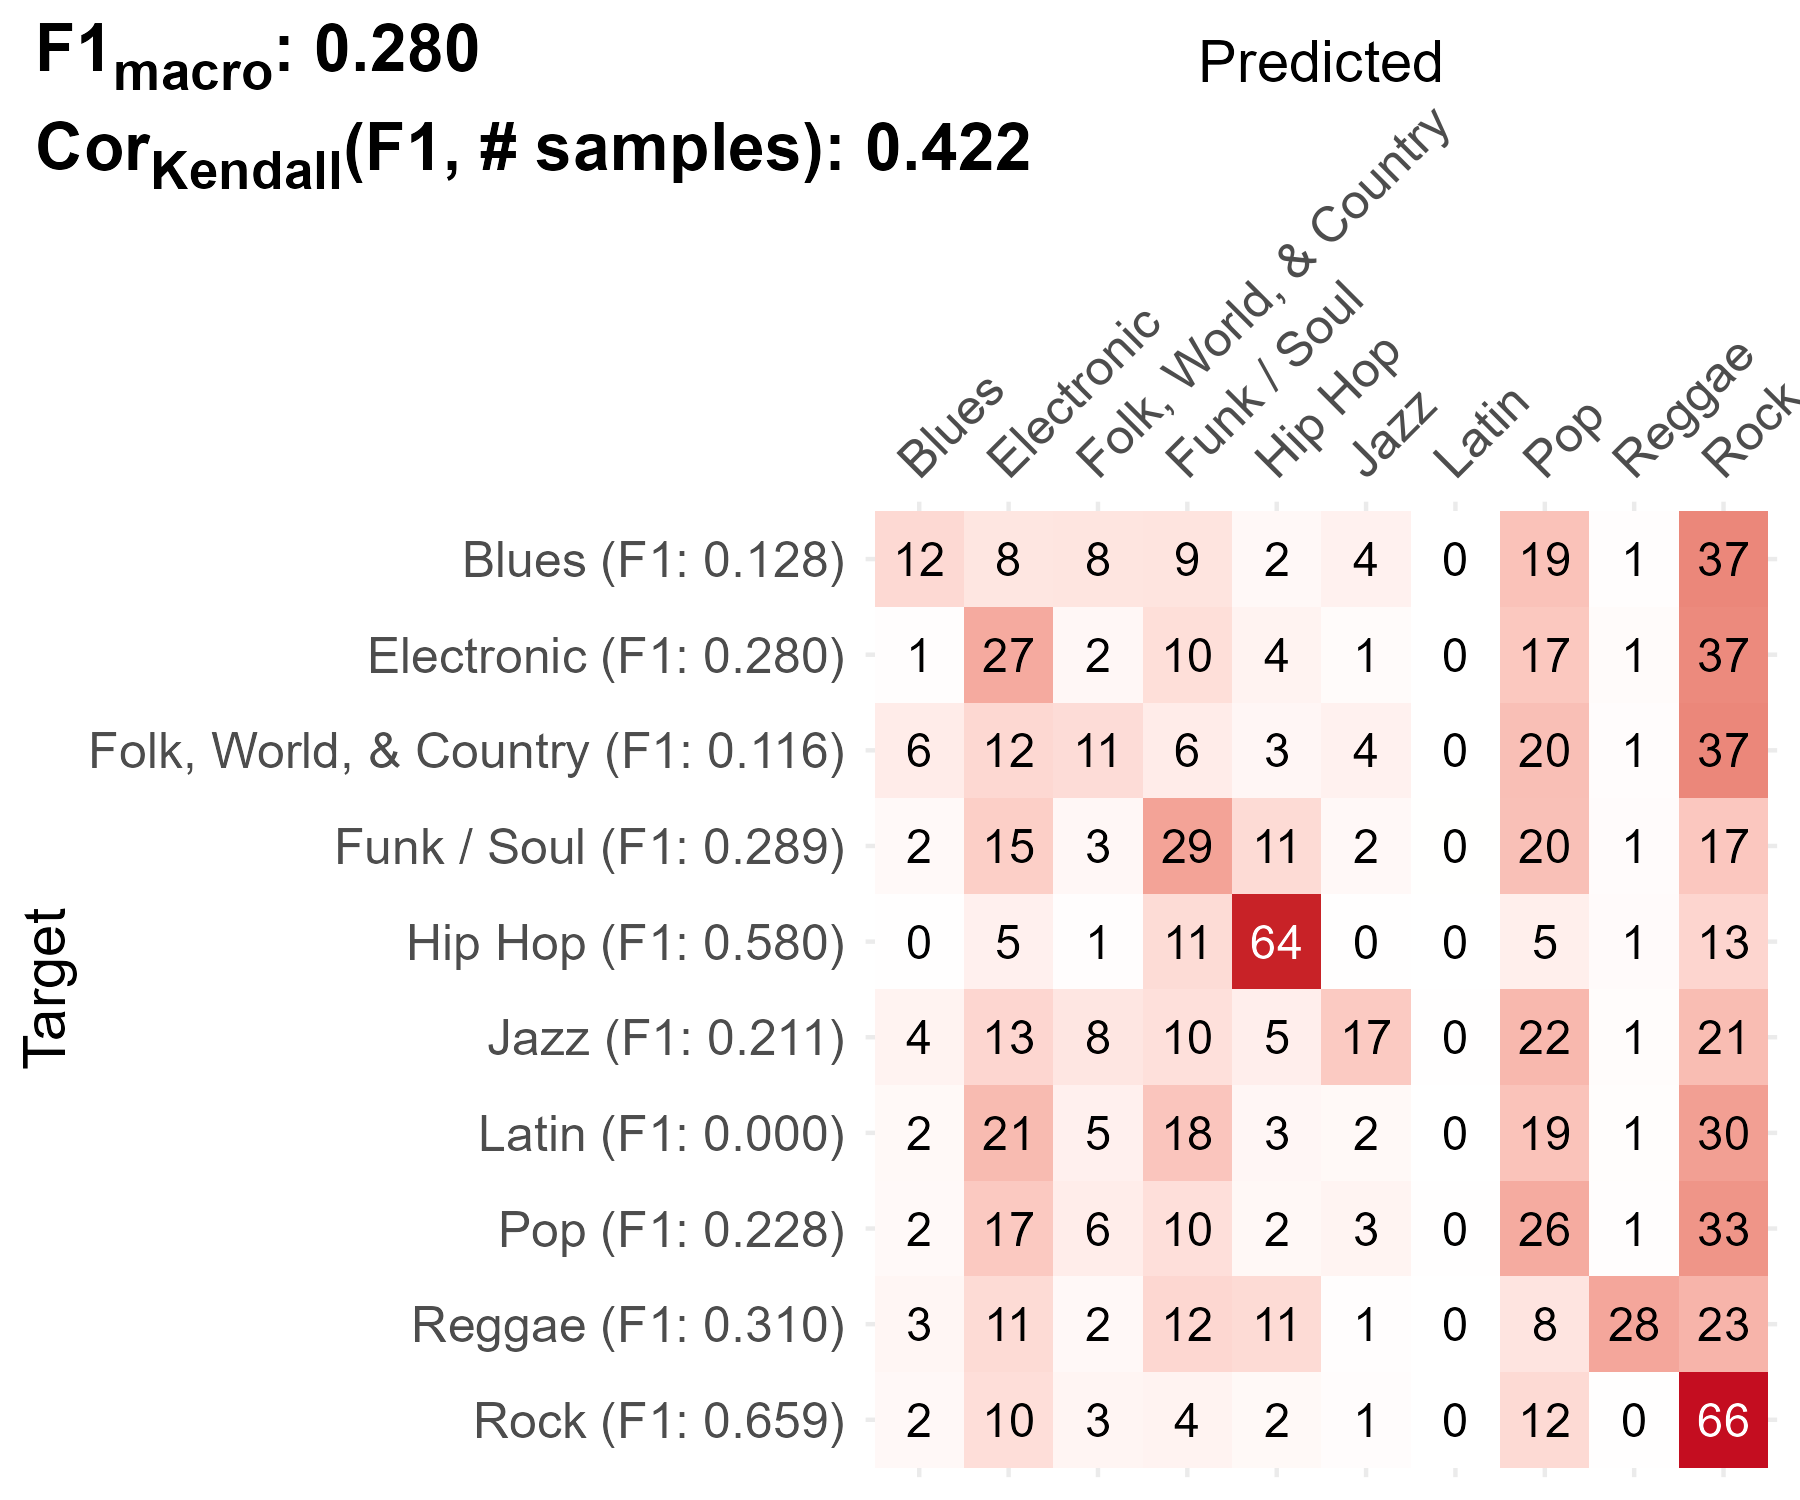
\includegraphics[alt={Confusion Matrix lightGBM},width=\linewidth]{figures/confusion_matrix.png}
  \caption{Confusion matrix for combined tuned lightGBM model [\%].}
  \label{fig:confusion_matrix}
\end{figure}


Using genre-discriminative topics, sentiments, and expression types as lyric features, we trained two machine learning models (GLMNET and LightGBM) to predict song genre based solely on lyrics. Their performance was compared to a random baseline, a traditional TF-IDF + GLMNET pipeline, and a DistillBERT model trained directly on raw lyrics. Structured-feature models underwent systematic hyperparameter tuning to ensure optimal parameterization. Table~\ref{tab:f1} reports macro F1 scores from 4-fold cross-validation and holdout evaluation.

Structured representations provided informative genre signal beyond uninformative baselines: the random model reached 0.111 and TF-IDF + GLMNET 0.248 on the holdout. DistillBERT achieved the highest overall performance (holdout $F1$=0.374), indicating the strength of contextual embeddings for lyric classification. Among structured features, expressions contributed most to genre discrimination (0.282), followed by topics (0.229) and sentiments (0.135). Combining all three improved performance, with GLMNET (C=1, L1=0.5) attaining 0.292 on the holdout, exceeding individual feature sets.

Hyperparameter tuning yielded further improvement. A regularized GLMNET (C=0.002, L1=0.33) achieved 0.335 in cross-validation and 0.291 on holdout, while the tuned LightGBM model performed best among structured approaches (CV 0.354, holdout 0.300). Although DistillBERT remained strongest overall, the tuned LightGBM retained approximately 80\% of its predictive power while employing interpretable features and interpretability regarding feature contributions.

When looking at the confusion matrix for the tuned combined features LightGBM model (see Figure \ref{fig:confusion_matrix}), we find that the model performs particularly well for \textit{Hip Hop} (holdout $F1$=0.591) and \textit{Rock} (0.584). The model performs worst for \textit{Folk, World \& Country} (0.177) and \textit{Jazz} (0.137). Off-diagonal confusions cluster among stylistically adjacent categories (e.g., \textit{Funk / Soul}, \textit{Pop}, and \textit{Electronic}; \textit{Hip Hop} and \textit{Funk / Soul}). While the results show a moderate positive relationship between genre prevalence and classification quality (Kendall correlation between per-genre F1 and sample size = 0.389); some genres with less samples (e.g., \textit{Hip Hop}) clearly outperform larger ones (e.g., \textit{Pop}).



% RQ3: What can we learn about lyrical genre differences from such interpretative models for popular music studies?
\subsection{Feature Importances and SHAP Values}
\begin{figure}
  \centering
  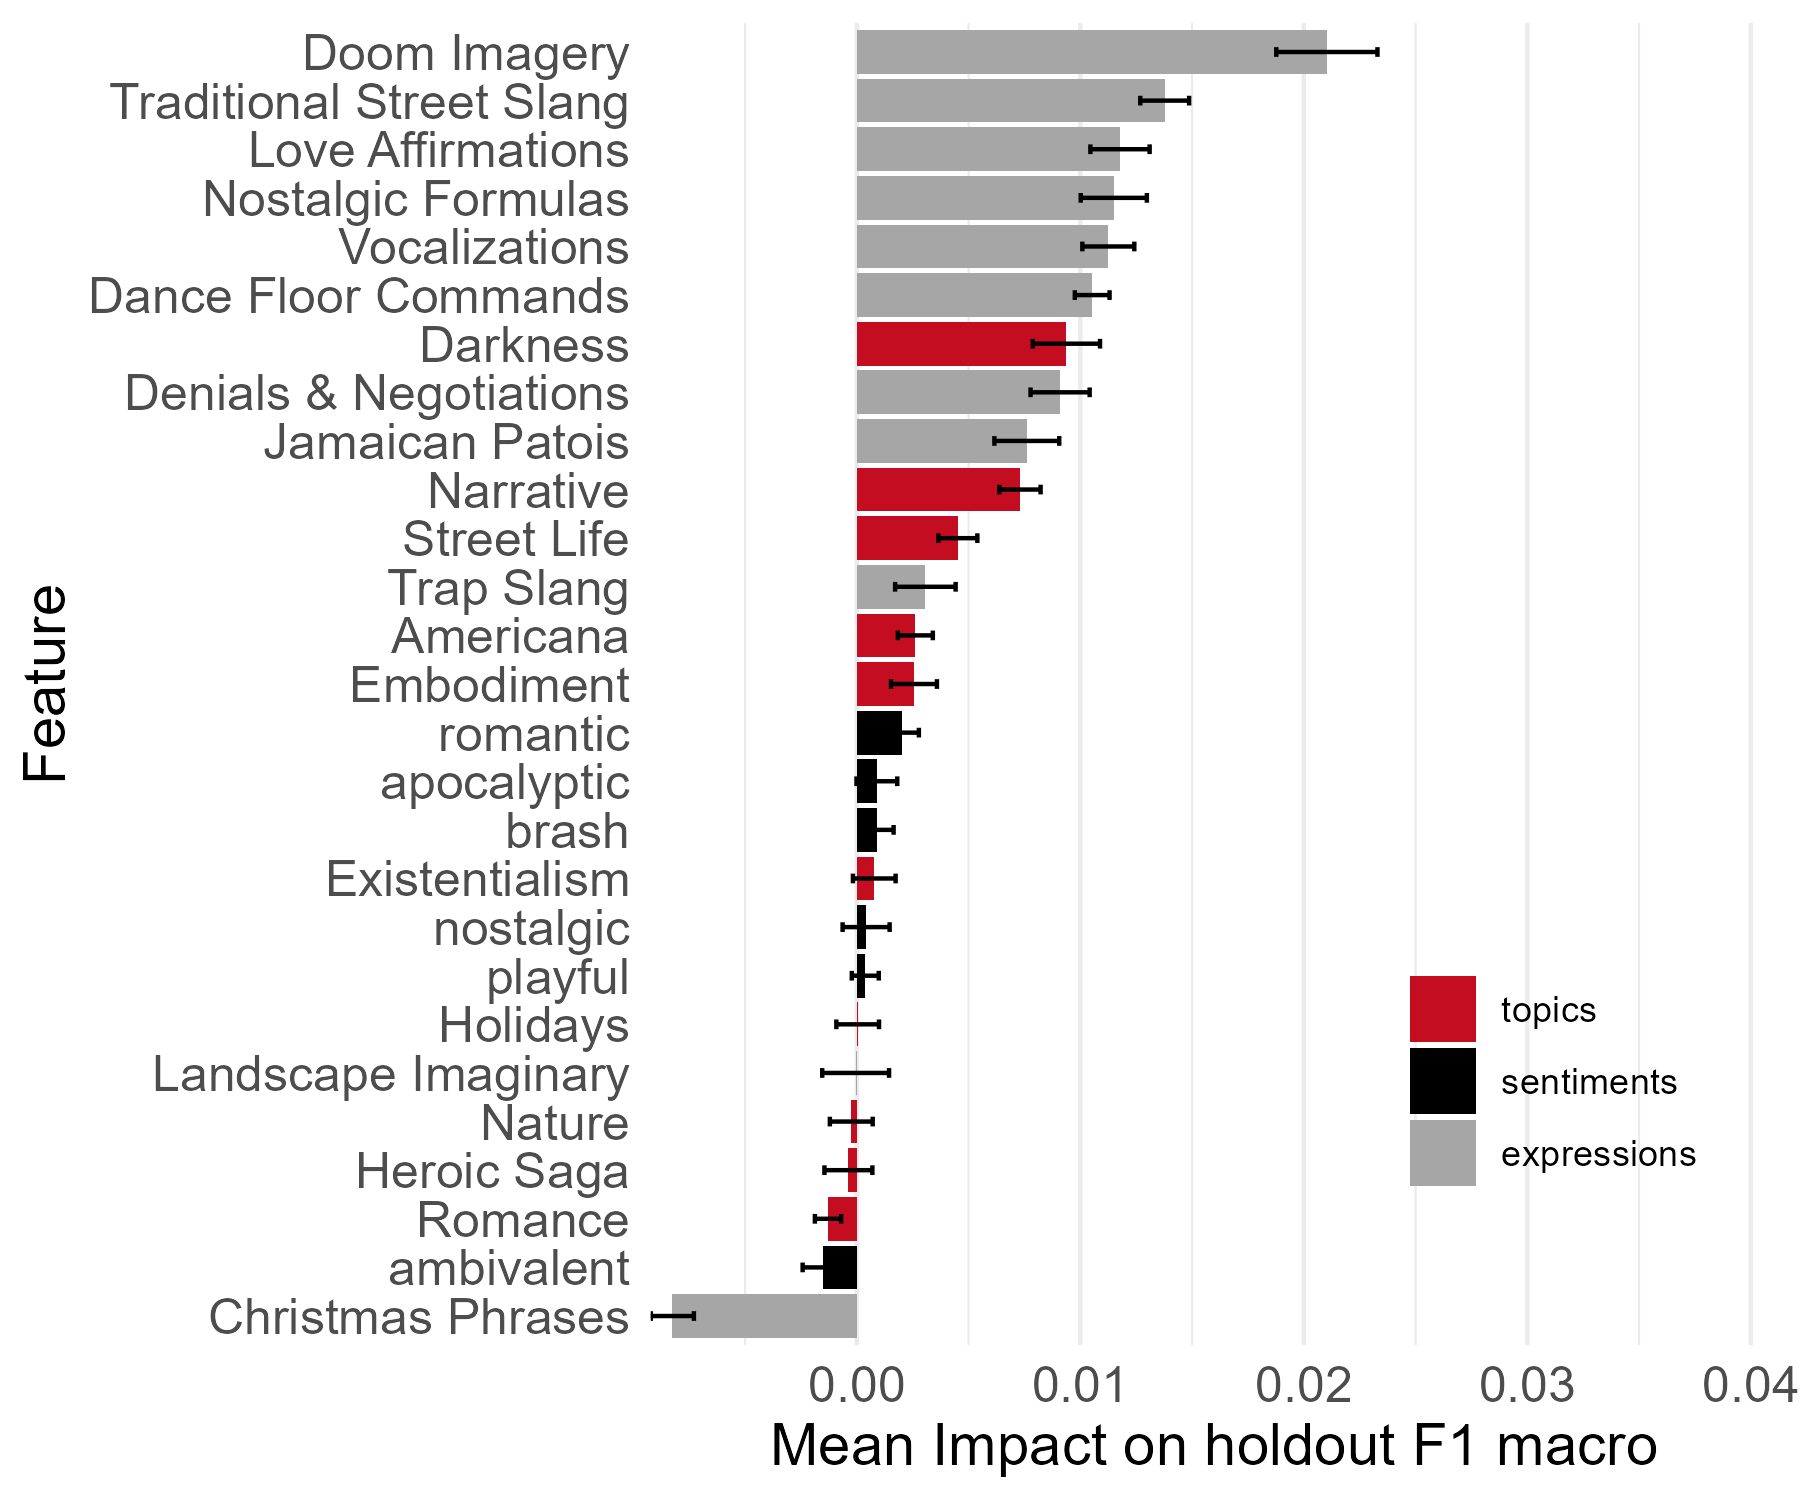
\includegraphics[alt={Permutation importance top 20 variables lightGBM},width=\linewidth]{figures/holdout_permutation_importance.png}
  \caption{Permutation importance on Heldout data for the tuned combined features LightGBM model.}
  \label{fig:permutation_importance}
\end{figure}

To assess which stylistic patterns shape music genre differentiation, we computed the permutation feature importance on the holdout set (Figure~\ref{fig:permutation_importance}). Expression-type features dominate the ranking: \textit{Doom Imagery}, \textit{Traditional Street Slang}, \textit{Love Affirmations}, \textit{Nostalgic Formulas}, \textit{Vocalizations} and \textit{Dance Floor Commands} emerged as the most influential predictors. Topic features such as \textit{Darkness}, \textit{Narrative}, and \textit{Street Life} occupied intermediate positions and produced moderate performance declines when permuted, suggesting that broader thematic context supports, but does not alone determine music genre distinction. Sentiment features showed only minor average impacts. The expression type \textit{Christmas Phrases} displays a clearly visible increase of holdout F1 when permuted, likely reflecting feature sparsity rather than substantive genre relevance.


\begin{figure}
  \centering
  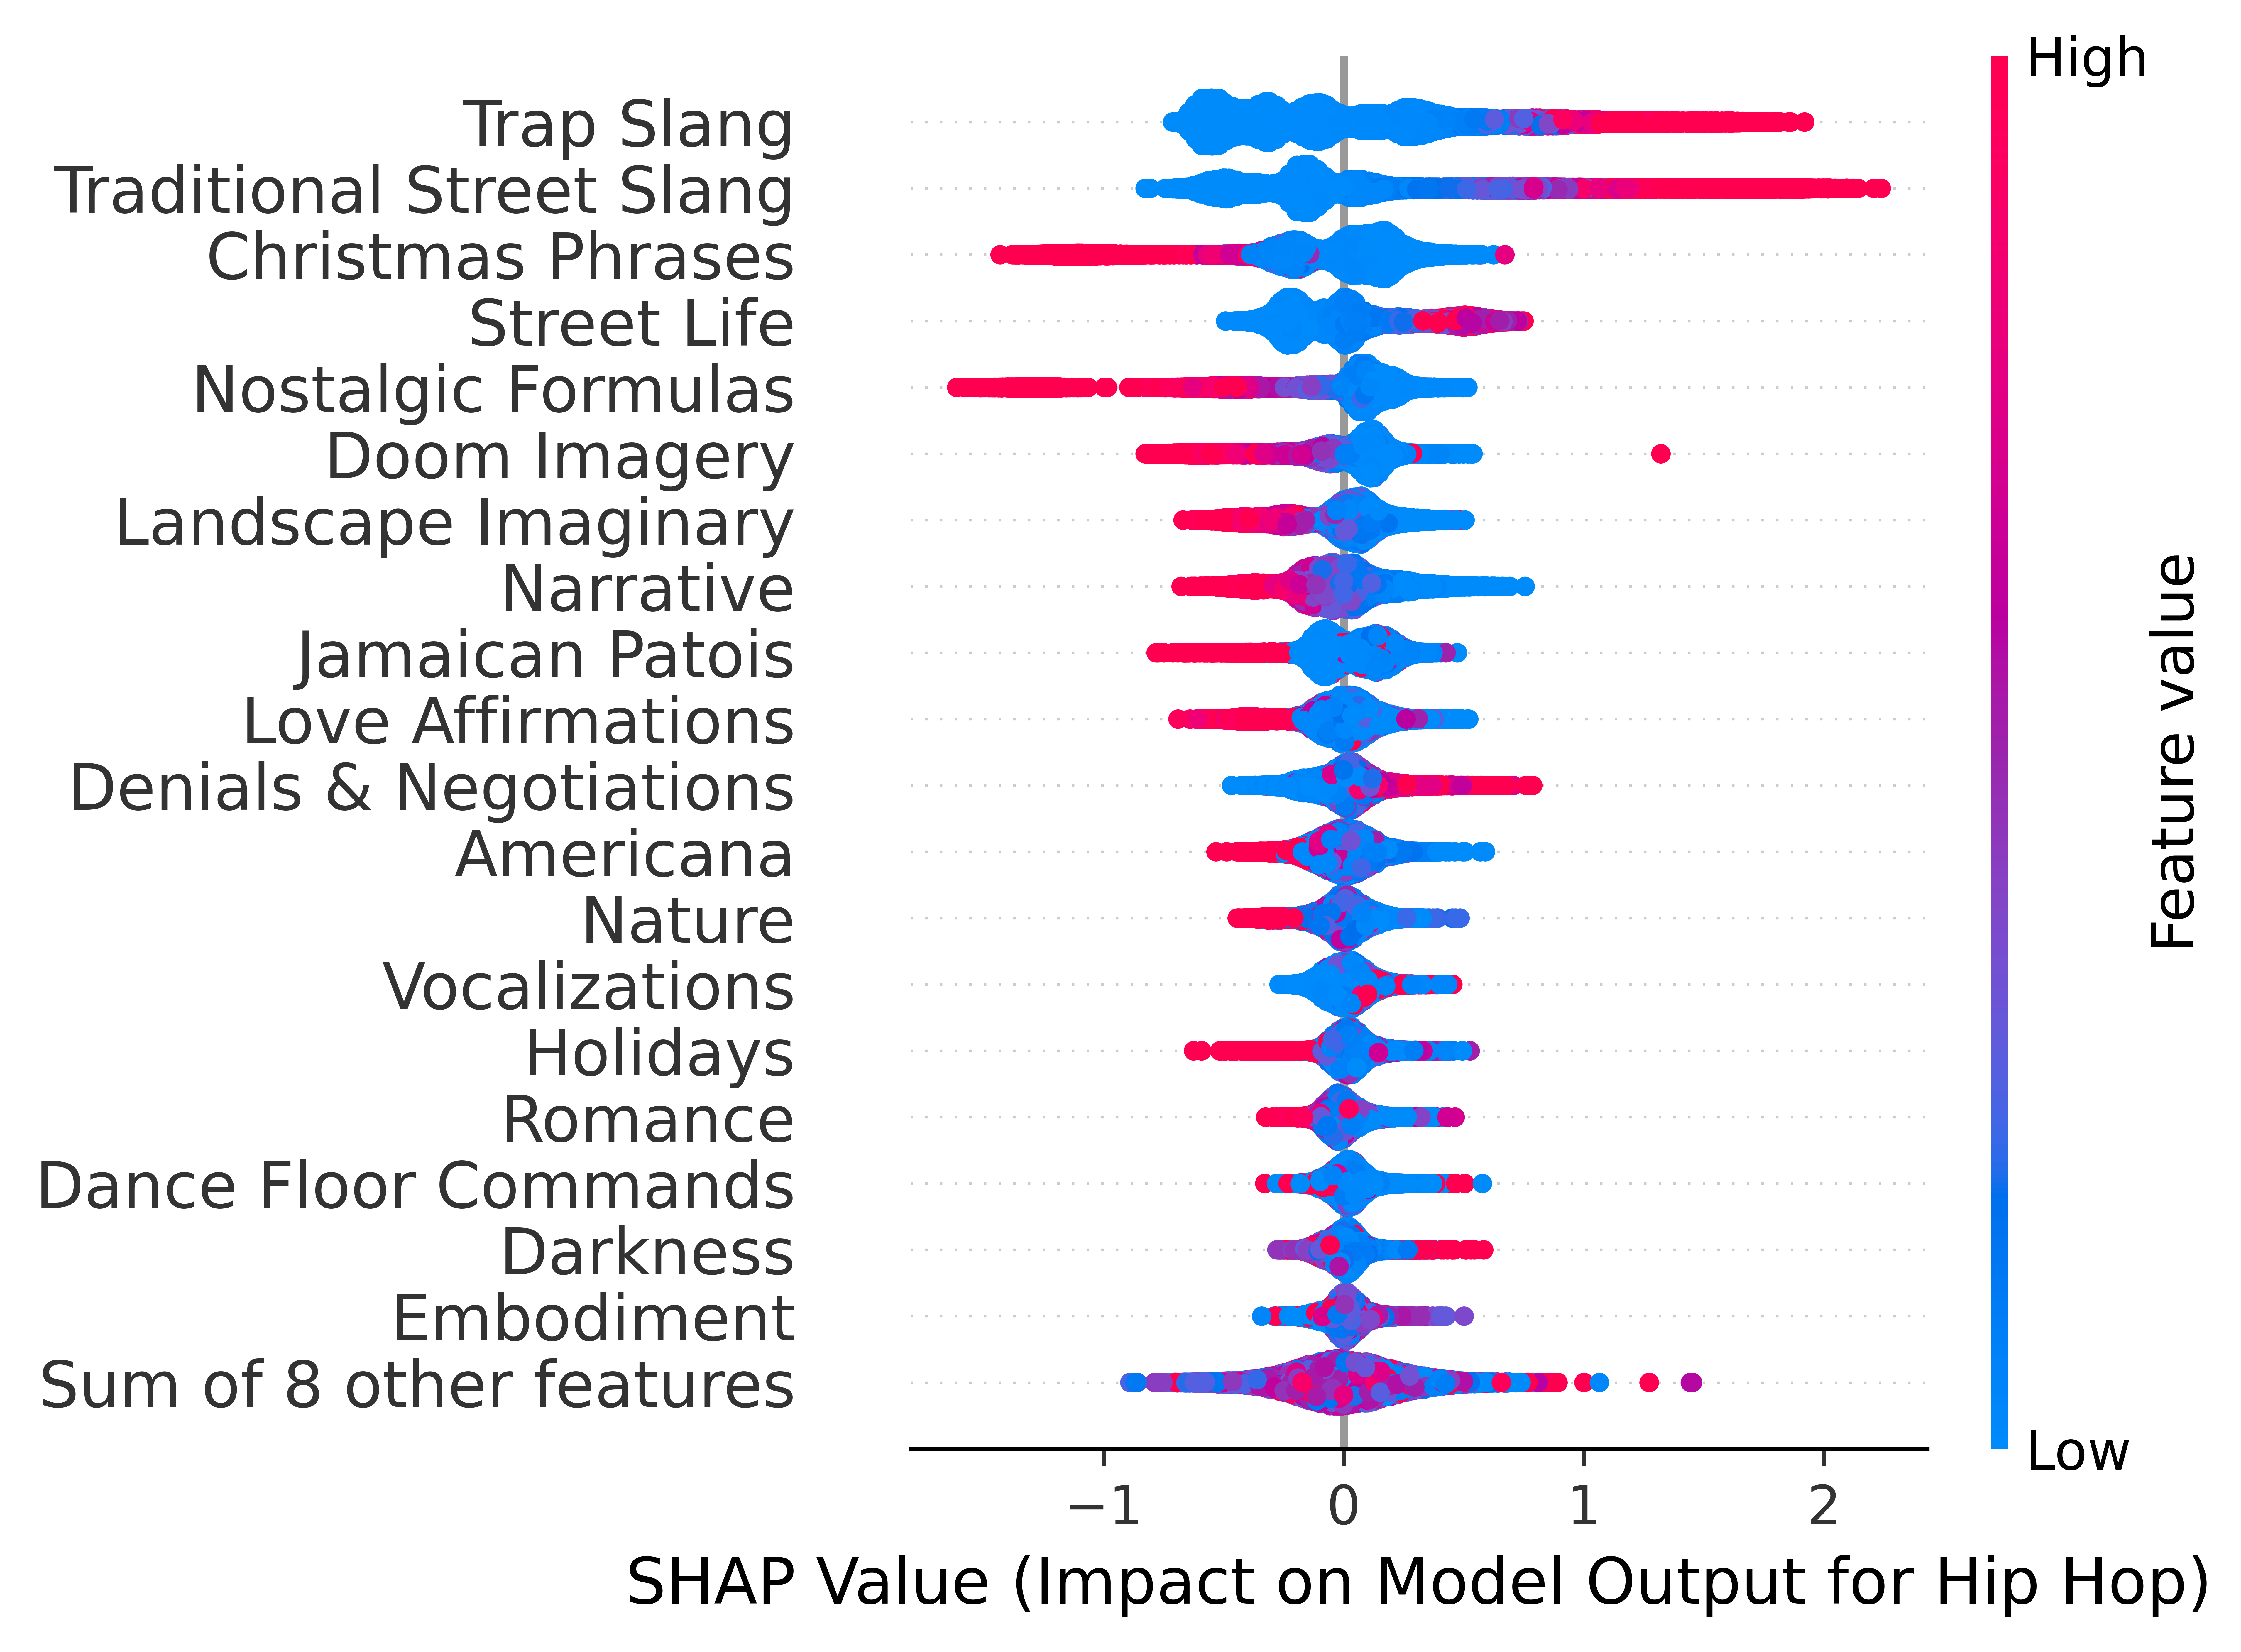
\includegraphics[alt={SHAP values for for Hip Hop prediction},width=\linewidth]{figures/shap_hip_hop.png}
  \caption{Example: SHAP values for \textit{Discogs' Hip Hop}.}
  \label{fig:shap_hip_hop}
\end{figure}

As an illustrative example of what interpretative models can reveal about lyrical genre differentiation, Figure~\ref{fig:shap_hip_hop} shows SHAP values computed on the holdout sample for the \textit{Hip Hop} class (holdout $F1$=0.591). High values for \textit{Trap Slang} and \textit{Traditional Street Slang} strongly increase the model's predicted \textit{Hip Hop} score; \textit{Street Life} and \textit{Denials \& Negotiations} similarly shift predictions toward this genre. In contrast, features such as \textit{Christmas Phrases} and \textit{Nostalgic Formulas} are associated with lower Hip Hop likelihoods. Some features (e.g., \textit{Doom Imaginary}, \textit{Jamaican Patois}, and \textit{Love Affirmations}) show more heterogeneous impacts, with high values sometimes increasing and sometimes decreasing \textit{Hip Hop} predictions, reflecting context-dependent effects. Sentiment features do not appear to among the most helpful features for \textit{Hip Hop} identification in our corpus.

\section{Discussion}
With this contribution, we identify genre-discriminative lyrical patterns in Anglophone German popular music (RQ1), including 10 topics, 6 sentiments, and 11 types of idiomatic expressions. Interpretable ML models based on these patterns (RQ2) retained 80\% of the predictive performance of a fine-tuned DistilBERT classifier, demonstrating that genre-discriminative lyrical pattern features can be effectively leveraged for genre classification while offering interpretability. Feature importance analyses (RQ3) revealed that idiomatic expressions play particularly important roles in genre discrimination, compared to topics and sentiments. Using \textit{Hip Hop} as an example, we show how specific types of expressions, topics, and sentiments characterize this genre in contrast to others. 

Lyrical genre distinction is driven not only by surface-level textual properties such as lyric length, vocabulary size, rhymes, echoisms, or readability (SOURCE), but also by content-related patterns identified in our analysis (RQ1). In particular, idiomatic expression types emerge as a more informative semantic dimension of genre differentiation than topics and sentiments (SOURCES). This suggests that genre-specific ways of phrasing meaning, rather than only thematic content or affective valence, contribute substantially to how genres are lyrically defined and perceived (SOURCE). These findings also support the view that genre cues operate across multiple linguistic levels (SOURCE).

For our interpretable ML experiments (RQ2), Hip Hop and Rock were among the genres that were most readily identifiable from lyrical features alone, suggesting that some genres rely more strongly on distinctive lyrical content markers, whereas others share more of these markers and are therefore more easily confused. Given, that \textit{Discogs' Rock} genre encompasses also metal styles, this is consistent with prior work on lyric-based genre classification (SOURCE) and with the idea of genre as a fuzzy category organized around prototypical rather than strictly necessary features (SOURCE). Importantly, we recover a substantial portion of the performance of a fine-tuned DistillBERT model using human-readable features, indicating that the transformer is exploiting structure that is at least partly accessible to interpretable textual analysis based on n-grams. These results suggest a division of labor in computational musicology: transformer models serve as high-performing baselines, whereas interpretable models are especially useful for assessing whether lyrical patterns generalize beyond the observed sample and for identifying which features reliably support genre discrimination in a way that remains linguistically interpretable (SOURCE).

Feature importance analysis (RQ3) reveals that genre differences in lyrics are primarily driven by idiomatic expression types such as \textit{Traditional Street Slang}, \textit{Trap Slang}, and \textit{Doom Imagery}, rather than emotional expression or thematic content alone. As illustrated by the \textit{Hip Hop} case, where street life topics and slang expressions jointly elevate genre predictions, these findings suggest that genres differ in how they package meaning through stylistic phrasing, with thematic content playing a supporting role (SOURCE). Instead of single defining markers, interactions between expression types, topics, and sentiments form profiles of lyrical content that encode genre identity. This aligns with a view of genre as a fuzzy, relational construct distinguished by bundles of linguistic cues meaningful in contrast to neighboring genres (SOURCE).

Taken together, these findings advance computational musicology by establishing a principled division between predictive and explanatory machine learning approaches. While transformer models excel at achieving high genre classification performance, interpretable models like ours reveal which linguistic patterns drive those predictions, enabling insights in lyrical genre formation rather than mere correlational tagging (SOURCE). This explanatory capacity supports practical applications including understanding genre biases in generative lyrics production models (SOURCE), where knowing that Trap Slang and Doom Imagery strongly signal specific genres can help identify and mitigate unintended stylistic skews in AI-generated content; corpus curation tools that automatically flag culturally distinctive lyrical markers for ethnomusicological analysis (SOURCE); and hybrid genre taggers for streaming platforms that balance predictive power with transparency for content moderation or artist discovery (SOURCE).
% TODO Topic modeling approach can also be used in music domain, as has been demonstrated by Mauch et al (2015)

Our analysis faces several limitations. First, music genre is inherently fuzzy, and by using 	\textit{Discogs} labels, we adopt a particular community's perspective on genre boundaries. While tracks often belong to multiple genres (SOURCE), we intentionally simplified this to a single-label classification problem to enable interpretable modeling. % needs justification?
Second, permutation feature importance can be biased by correlated features. Although some of our features showed correlation, we chose not to cluster them beforehand to preserve the interpretability of individual linguistic patterns at the cost of potential ranking distortion. Finally, our corpus focuses on Anglophone popular music consumed in Germany, limiting generalizability to global Anglophone repertoires or non-English music popular in Germany.

Future research will extend this approach to other languages within the corpus, comparing lyrical patterns across linguistic contexts and exploring language-agnostic interpretable models. We also plan to test generalizability across diverse corpora beyond German popular music listening. Finally, we aim to incorporate additional lyrical features alongside multimodal audio and video characteristics to build more robust interpretable genre classifiers and examine interactions between lyrical patterns and other modality-specific genre cues.



\cite{monroeFightinWordsLexical2017} %only for compiling not to fail



% \section{Acknowledgments}
% Only to include in the camera-ready version. Does not count towards the page limit.

\section{AI Usage Statement}
See submission guidelines. Does not count towards the page limit.

% For BibTeX users:
\bibliography{refs}

% For non BibTeX users:
%\begin{thebibliography}{citations}
% \bibitem{Author:17}
% E.~Author and B.~Authour, ``The title of the conference paper,'' in {\em Proc.
% of the Int. Society for Music Information Retrieval Conf.}, (Suzhou, China),
% pp.~111--117, 2017.
%
% \bibitem{Someone:10}
% A.~Someone, B.~Someone, and C.~Someone, ``The title of the journal paper,''
%  {\em Journal of New Music Research}, vol.~A, pp.~111--222, September 2010.
%
% \bibitem{Person:20}
% O.~Person, {\em Title of the Book}.
% \newblock Montr\'{e}al, Canada: McGill-Queen's University Press, 2021.
%
% \bibitem{Person:09}
% F.~Person and S.~Person, ``Title of a chapter this book,'' in {\em A Book
% Containing Delightful Chapters} (A.~G. Editor, ed.), pp.~58--102, Tokyo,
% Japan: The Publisher, 2009.
%
%\end{thebibliography}

\end{document}
